\section{A framework for efficient GPU implementations of collision attacks}

In the previous section, we have described the framework used to mount freestart collision attacks on \shaone. We now turn to
the matter of concrete implementation of the attack procedure. Specifically, we describe implementations on \emph{graphics processing
units} (GPUs).

The use of GPUs is attractive for computation-intensive cryptanalysis, as they offer much more raw computational power than
similarly-priced general-purpose processors (CPUs). The availability of efficient frameworks for general-purpose GPU programming such as CUDA~\cite{cuda} allows
for potentially complex code to be conveniently deployed on GPUs. However, the differences in architecture between CPUs and GPUs
as highlighted below need to be taken into account, and not every attack may be suitable for a GPU implementation.

GPUs have already been used with some success in heavy-computation cryptography, notably to aid in integer factorization or in finding discrete
logarithms~\cite{DBLP:conf/asiacrypt/BosK12,DBLP:conf/ches/MieleBKL14,DBLP:conf/eurocrypt/BarbulescuGGM15,DBLP:phd/hal/Jeljeli15}, and also for collision attacks on reduced \shaone~\cite{cryptoeprint:2011:641}.
Even if the latter case in particular is essentially identical to our own, we nonetheless developed our GPU framework for implementing collision attacks from scratch.

\subsection{GPU architecture and programming model}

We start by first recalling a few important points about current GPUs that will help
understanding our design decisions. We specifically discuss these points
for Nvidia GPUs of the \emph{Maxwell} generation such as the \gtx
used in our attacks.

%\paragraph{Number of cores and scheduling.}
A modern GPU can feature more
than a thousand small cores, that are packed together in a small
number of larger ``multiprocessor'' execution units. Taking the example of the
Nvidia \gtx for concreteness, there are 13 multiprocessors of 128 cores each,
making 1664 cores in total~\cite{gtx970_specs}. The fastest instructions
such as for instance 32-bit bitwise logical operations or modular addition have a throughput of 1 per core,
which means that in ideal conditions 1664 instructions may be simultaneously processed by such a GPU in one clock
cycle~\cite{cuda_prog_guide}.

Yet, so many instructions cannot be emitted independently, or to put it in another way, one cannot run an independent
thread of computation for every core. In fact, threads are grouped together by 32 forming a \emph{warp}, and only
warps may be scheduled independently. Threads within a warp may have a diverging control flow, for instance by
taking a different path upon encountering a conditional statement, but their execution in this case is
serialized. At an even higher level, warps executing the same code can be grouped together as \emph{blocks}.

%Furthermore, on each multiprocessor one can run up to 2048 threads simultaneously, which are dynamically scheduled every cycle
%onto the 128 cores at a warp granularity.
%Thus while a warp is waiting for the results of a computation or for a (high latency) memory operation to return,
%another warp can be scheduled.
%Although having more threads does not increase the computational power of the multiprocessor, such overbooking of cores can be used to hide latencies and thus increase efficiency of a GPU program.
%
%In short, to achieve an optimal performance, one must bundle computations by groups of 32 threads executing
%the same instructions most of the time and diverging as little as possible and use as many threads as possible.

Each multiprocessor can host a maximum of 2048 threads regrouped
in at least 2 and at most 32 blocks~\cite{cuda_prog_guide}. If every multiprocessor of the GPU hosts 2048 threads, we say that we have
reached \emph{full occupancy}. While a multiprocessor can only physically run one thread per core, \ie 128, at a given time,
a higher number of resident threads is beneficial to hide computation and memory latencies.
These can have a significant
impact on the performance as a single waiting thread causes its entire warp of 32 to wait with him; it is thus important in
this case for the multiprocessor to be able to schedule another warp in the meantime.

Achieving full occupancy is not however an absolute objective as it may or may not result in optimal performance depending on the
resources needed by every thread. Important factors in that respect are the average amount of memory and the number of registers
needed by a single thread, both being resources shared among the threads.
In our implementation, the threads need to run rather heavy functions and full occupancy is typically
not desirable. One reason why it is so is that we need to allocate 64 registers per thread in order
to prevent register spilling in some of the most expensive functions; a multiprocessor
having ``only'' $2^{16}$ registers, this limits the number of threads to 1024. As a result, we use a layout of
26 blocks of 512 threads each, every multiprocessor being then able to host 2 such blocks.

\bigskip

%\paragraph{Memory architecture and thread synchronization.}
In the same way as they feature many execution units, GPUs also provide
memory of a generous size, \eg 4 GB for the \gtx, which must however be shared among the threads. The amount of memory available to a single thread
is therefore much less than what is typically available on a CPU; though it of course highly depends on the number of
running threads, it can be lower than 1\,MB. This, together with the facts that threads of a same warp do not actually execute
independently of each other and that threads of a same block run the same code makes it enticing to organize the memory
structure of a program at the block level. Fortunately, this is made rather easy by the fact that many efficient
synchronization functions are available for the threads, both at the warp and at the block level.

\subsection{High-level structure of the framework}

%\paragraph{Balancing the work between the GPU and the CPU.}
The implementation of our attacks can be broadly decomposed into two phases. The first step consists in computing a certain number
of base solutions and in storing them on disk.
Because the total number of base solutions necessary to find a collision
is rather small (about $2^{25}$ in the 76-step case, for instance) and because they can be computed
quickly, this can be done efficiently in an offline fashion using CPUs.

The second phase then consists in trying to extend probabilistically the base solutions to satisfy path conditions up to a further point by
trying many neutral bit combinations, in the hope of eventually finding a collision.
This is an intensely parallel task that is well suited to running on GPUs. However, as it
was emphasized above, GPUs are most efficient when there is a high coherency between the execution of many threads. For that reason,
we must avoid having idle threads that are waiting because their candidate solutions failed to follow the differential paths, while
others keep on verifying a more successful one. Our approach to this is to fragment the verification into many small functions
or \emph{snippets}
that are chosen in a way which ensures that coherency is maintained for every thread of a warp when executing a single snippet, except in
only a few small points. This is achieved through a series of intermediary buffers that store inputs and outputs for the snippets.
A warp then only executes a given snippet if enough inputs are available for every of its threads.
One should note that there is no need to entirely decompose the second step of the attack into snippets, and that a final part can again
be run in a more serial fashion, typically on CPU. Indeed, if inputs to such a part are scarce, there is no real advantage in verifying them in
a highly parallel way.


The sort of decomposition used for the GPU phase of our attack as described above is in no way constrained by the specific context of a \shaone collision search.
In fact, it is quite general, and we believe that it can be successfully applied to many an implementation of (symmetric) cryptographic
attacks. We conclude this section by giving more details of the application of this approach to the case of \shaone.

%\paragraph{Choice of the snippets.}

\bigskip

As we mentioned in \autoref{sec:framework}, the attack process consists in trying many combinations of neutral bits, with each step in a small window
adding new neutral bits to be tested. It is thus quite natural to reflect this process in the choice of the snippets:
we use intermediary buffers to store partial solutions up to $\state_{17}$ (\ie base solutions), $\state_{18}$, etc.
Then for each step the corresponding snippet consists
in loading one partial solution per thread of a warp and applying every possible combination of neutral bits for this step. Each combination
is tried by every thread at the same time on its own partial solution, thereby maintaining coherency.
Then, each thread assesses if the current combination yields a valid extension by one step of its own partial solution, and writes the result to
an output buffer for the snippet, which is the input buffer for the next snippet, if this is the case;
this conditional write is the only part of the code where threads may briefly diverge.

For the
later steps when no neutral bits can be used anymore, the snippets regroup the computation of several steps together.
Eventually the verification that partial solutions up to step 56 (in the 76-step case; 60 in the 80-step one) result in valid collisions is done on a CPU. This is partly because
the amount of available memory makes it hard to use step-by-step snippets until the end, but also because such partial solutions are only
produced very slowly. For instance, a single \gtx produces partial solutions up to step 56 of a 76-step collision at a speed of about 0.017 solution per second, that is about
1 per minute; waiting for enough partial solutions to feed a single complete warp would in this case take a completely unreasonable half hour.

\bigskip


%\paragraph{Complete process of the attack.}
A complete implementation of an attack mostly consists in the snippets and supporting functions, such as buffer management.
Connecting the snippets together is straightforward. Every warp tries to work with partial solutions that are up
to the latest step for which enough solutions are available. This means that it visits the buffer of partial solutions in order from the top,
stopping at the first that is able to feed it entirely.
In the worst case where none of the buffers are full enough, it simply resorts to using base solutions.

In practice, warps spend most of their time feeding on partial solutions that are valid up to a rather late step. For instance, in the 76-step attack,
about 90\% of the time is spent on $\state_{24}$ or higher, which is at most two steps away from the latest one where neutral bits are available.
Thus, work on early steps and in particular on base solutions is done only intermittently.

We conclude this high-level description by giving a simplified flow chart
of the GPU part of the 76-step attack in \autoref{fig:attack_diagram}, made slightly incorrect for the sake of clarity, notably omitting the fact that further verification is still done on GPU up to steps 56.

\def\rectanMac{\begin{tikzpicture}[scale=0.2]\draw (0,0) rectangle (1,1);\end{tikzpicture}}
\def\elliMac{\begin{tikzpicture}[scale=0.3,transform shape]\node[draw,ellipse] (e) at (0,0) {\phantom{toto}};\end{tikzpicture}}
\def\plainMac{\begin{tikzpicture}[scale=0.1] \draw[>=latex,->] (0,0) -- (2,2);\end{tikzpicture}}
\def\dottMac{\begin{tikzpicture}[scale=0.1] \draw[dotted,->]   (0,0) -- (2,2);\end{tikzpicture}}

\begin{figure}[htb]
%%\begin{sideways}
%%%%%% EPRINT %%%%%
%% Minipage changed to 6cm from 5cm
%\begin{minipage}{6cm}
  \begin{center}
% Figure scale changed from .68. Set that back for proceedings
  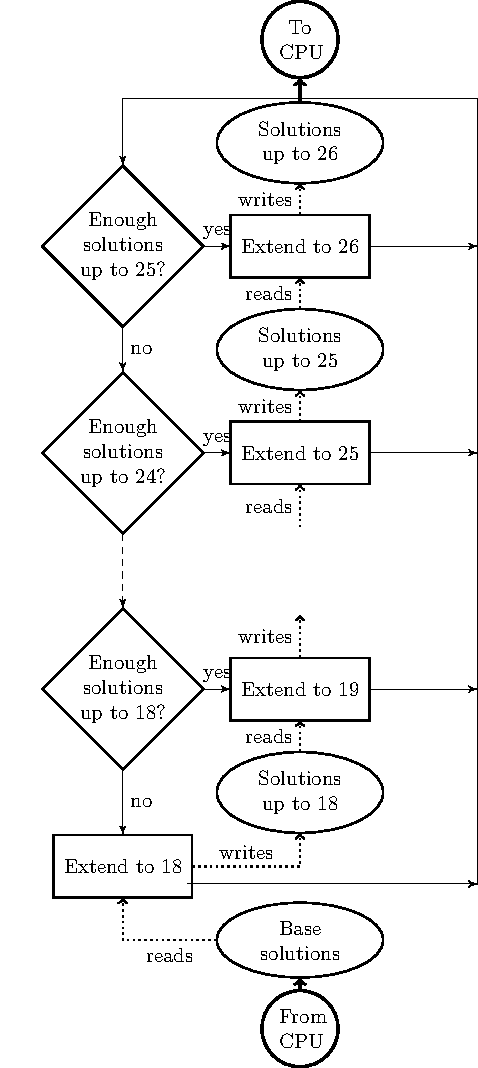
\includegraphics[scale=0.7]{figures/attack_diagram_std.pdf}
%%%%% /EPRINT %%%%
  \end{center}
%\end{minipage}
%\end{sideways}
  \caption[Simplified flow chart for the GPU part of the attack.]{Simplified flow chart for the GPU part of the attack. The start of this infinite loop is
  in the top left corner. Rectangles ``\,\protect\rectanMac\,'' represent
  snippets, ellipses ``\,\protect\elliMac\,''
  represent shared buffers, plain lines ``\,\protect\plainMac~''
  represent control flow, and dotted lines ``\,\protect\dottMac~'' represent data flow.}
  \label{fig:attack_diagram}
\end{figure}


\subsection{Implementation details}

We now give more details about the implementations of the attacks. In particular, we discuss
how partial solutions are represented at various steps in \autoref{sec:part_sol} and
we comment the code of a snippet function in \autoref{sec:snippet}. We very briefly discuss how
to tune GPU settings to use them more efficiently in \autoref{sec:gpu_tune}.

\subsubsection{Representation of partial solutions}
\label{sec:part_sol}

As the basis of our framework is to store, load and extend many partial solutions for the differential path, we need to be able to work with such objects
in an efficient way. One thus needs to define good representations for partial solutions, such that processing them is computationally simple, and managing them
in memory causes as little overhead as possible.

The representation we use is based on two types of buffers: some are holding enough information to define a \sha computation in its entirety, \ie it
contains the value of at least five (resp. sixteen) consecutive state (resp. message) words, while others only contain the necessary information to
express how the associated partial solution differs from a completely-defined one. Typically, the first kind of buffer may be used to store base solutions,
while the second is used to keep track of which neutral bits are active in a partial solution.

It is quite straightforward to define the structure of a base solution buffer, as there is little doubt about the necessary information they need
to include and the way to represent it. For instance, the 76-step base solution buffer contains the value of state words $\state_{13},\ldots,\state_{17}$
and of the message words $\expmess_6,\ldots,\expmess_{21}$. Additionally, it includes the value of $\state_{12}$; while this information is
not strictly necessary, it is useful to speed-up the computation of the activation of some neutral bits. Similar buffers without an extra state word
are used to hold partial solutions up to $\state_{36}$ and $\state_{56}$ (resp. $\state_{40}$ and $\state_{60}$ in the 80-step case). The choice
of these boundaries to define the late partial solutions were no more control is possible simply comes from the fact that a pair of messages following
the differential path of either attack is not expected to have any state differences at these steps. It is thus particularly efficient to filter
solutions that are not valid at these points.

The structures of the other buffers are also quite simple, but their instantiations may require some care to make them especially efficient.
In a nutshell, we just want such a buffer to keep a reference to a base solution and to remember the values of the currently active neutral bits.
To make this efficient and convenient to use, we would like to share a similar structure for the input and output buffers of a snippet; this would
allow to extend a partial solution that possibly already has some bits active by simply adding the newly activated bits for this step. This is the
approach we followed in our implementations, with an added refinement.

\medskip

We have already mentioned in the past section that \eg the 76-step attack contains neutral bits acting on a wide range of steps, from $\state_{18}$
to $\state_{26}$; the range for the 80-step attack is even wider, due to the use of boomerangs. Additionally, the neutral bits themselves are located on many message
words. Thus, it would seem wasteful to recompute the action of past neutral bits on message words as low as $\expmess_{14}$ while in the snippet corresponding
\eg to $\state_{24}$. Consequently, we have a strong incentive to store intermediary partial solutions in order to save some of this recomputation.

In the 76-step case, there is a natural location that may be used to define what we call \emph{extended base solutions}. As we will detail in
\autoref{sec:res_76}, neutral bits located on words $\expmess_{14}$ to $\expmess_{18}$ are only used up to $\state_{21}$, and the ones located
on words $\expmess_{19}$ to $\expmess_{21}$ are only used in later steps. Thus, it would make sense that once the active bits up to
$\expmess_{18}$ have all been determined, only the modified message words and the corresponding value for the state should be stored. There is
however no need to keep again sixteen message words in such an extended base solution, as most of them are identical to the ones of the corresponding
base solution, and as a base solution is in general extended into many distinct extended base solutions, it would not make sense to \eg add enough
message words to the latter and erase the former. One subtlety in the definition of this extended base solution is that
it also includes the message word $\expmess_{20}$. Although no neutral bits on this word
have been activated at the point where the solution is
formed, some of its bits may need to be flipped depending on the use of neutral bits on words $\expmess_{15}$ and $\expmess_{16}$, so as to
preserve message bit relations. A convenient way to remember this information is simply to preemptively add the possible contributions of the neutral
bits to $\expmess_{20}$ and to store this modified word in the extended base solution.
All in all, the buffer of extended base solution of the 76-step attack is made of twelve words: five state words $\state_{17}$ to $\state_{21}$,
six message words $\expmess_{14}$ to $\expmess_{18}$ and $\expmess_{20}$, and one word holding an identifier for the base solution from which
it is extended.

The ``inter-snippet'' buffers that refer to changes from a base or extended base solution are only made of two words consisting of concatenated
segments of the message words containing neutral bits and of a reference to the associated solution.

The 80-step attack uses similar representations but with a few variations. As we will show in \autoref{sec:res_80}, there are
more possible corrections on the messages to be performed in the 80-step attack to preserve message bit relations. Consequently, some of the precomputations of
individual neutral bit contributions are stored alongside the actual neutral bits. It is also slightly less immediate to determine where to
start defining an extended base solution, as there is no natural separation between the location of various neutral bits as there was in
the 76-step case. This is not a major issue, however, as the location of the neutral bits of a same word shared between base and extended base solutions
are not overlapping inside the word itself; splitting their representation over multiple buffers thus does not result in significant overhead.
Finally, the additional use of boomerang neutral bits, or somehow equivalently the use of more neutral bits than in the 76-step attack,
implies that the last inter-snippet buffers contain one more word  compared to the ones for early snippets and all such buffers
in the 76-step case, \ie three in total.

In \autoref{sec:res_76} and \autoref{sec:res_80}, we will describe the full content of most of the inter-snippet buffers.

\bigskip

We conclude this part by discussing some implementation aspects of the various buffers.

All of the buffers are cyclic and hold $2^{20}$ elements, regardless of their sizes, except the buffers of partial solutions extended up to
$\state_{36} \sim \state_{40}$ and $\state_{56} \sim \state_{60}$ which only have $2^{10}$ elements as they see a lower production rate due to their purely probabilistic nature.

With the exception of the buffers holding the base solutions and the collision candidates formed by partial solutions
up to $\state_{56} \sim \state_{60}$, \ie the buffers that are written or read by a CPU,
there is one instance of every buffer per block, \ie 26 buffers per GPU. This allows to use block-wise instead of global
synchronization mechanisms when updating the buffers' content,
thence reducing the overhead inherent to the use of such shared data structures.
Taken together, the buffers thus use a significant portion of the 4\,GB memory available on the \gtx, needing in the neighbourhood of 3\,GB.

We carefully took into account the presence of a limited amount of
very fast multi\-processor-specific shared memory. While the 96\,KB available per multiprocessor is
hardly enough to store the whole buffers themselves, we take advantage of it by dissociating the storage of
the buffers and of the meta-data used for their control logic, the latter being held in
shared memory. This improves the overall latency of buffer manipulations, especially in case of
heavy contention between different warps. This local shared memory is also very useful to buffer
the writes to the buffers themselves. Indeed, only a fraction of the threads of a warp often as low as $2^{-3}$
have a valid solution to write after having tested a single candidate,
and the more unsuccessful threads need to wait while the former write their solution to global memory.
It is therefore beneficial to first write the solutions to a small local warp-specific buffer and to
flush it to the main block-wise buffer as soon as it holds 32 solutions or more, thence
significantly reducing the number of accesses to the slower global memory.


\subsubsection{An example of snippet function}
\label{sec:snippet}

We now illustrate the discussion of this section by providing a commented snippet from the 76-step attack given in \autoref{lst:snippet_example} written in \textsf{CUDA C/C++}, namely a function that is taking partial solutions up to $\state_{22}$  and that is
trying to extend them up to $\state_{23}$ using neutral bits on $\expmess_{19}$. Its structure is a straightforward application of the framework, and is fairly representative of most of the
code of both of our attacks although some snippets may at first seem more complex due to their use of neutral bits located on several distinct message words.

\begin{minted}[linenos,breaklines]{c}
__device__ void stepQ23(uint32_t thread_rd_idx)
{
	uint32_t base_idx = Q22SOLBUF.get<11>(thread_rd_idx);
	uint32_t q17 = Q22SOLBUF.get<0>(thread_rd_idx);
	uint32_t q18 = Q22SOLBUF.get<1>(thread_rd_idx);
	uint32_t q19 = Q22SOLBUF.get<2>(thread_rd_idx);
	uint32_t q20 = Q22SOLBUF.get<3>(thread_rd_idx);
	uint32_t q21 = Q22SOLBUF.get<4>(thread_rd_idx);
	uint32_t m6  = BASESOLBUF.get<6>(base_idx);
	uint32_t m8  = BASESOLBUF.get<8>(base_idx);
	uint32_t m19 = BASESOLBUF.get<19>(base_idx);
	uint32_t m21 = BASESOLBUF.get<21>(base_idx);
	uint32_t m14 = Q22SOLBUF.get<5>(thread_rd_idx);
	uint32_t m22;

	uint32_t q22  = sha1_round2(q21, q20, q19, q18, q17, m21);

	uint32_t w19_q23_nb = 0;
	for (unsigned i = 0; i < 32; i++)
	{
		NEXT_NB(w19_q23_nb, W19NBQ23M);

		m19 &= ~W19NBQ23M;
		m19 |= w19_q23_nb;
		m22 = sha1_mess(m19, m14, m8, m6);

		uint32_t newq20 = q20 + w19_q23_nb;
		uint32_t newq21 = q21 + rotate_left(w19_q23_nb, 5);
		uint32_t newq22 = sha1_round2(newq21, newq20, q19, q18, q17, m21);
		uint32_t newq23 = sha1_round2(newq22, newq21, newq20, q19, q18, m22);

		uint32_t q23nessies = Qset1mask[QOFF + 23] ^ (Qprevrmask [QOFF + 23] & rotate_left(newq22, 30));
		bool valid_sol = (0 == ((newq21 ^ q21) & Qcondmask[QOFF + 21]));
		valid_sol &= (0 == ((newq22 ^ q22) & Qcondmask[QOFF + 22]));
		valid_sol &= (0 == ((newq23 ^ q23nessies) & Qcondmask[QOFF + 23]));

		uint32_t sol_val_0 = pack_update_q23_0(m19);
		uint32_t sol_val_1 = pack_update_q23_1(thread_rd_idx);

		WARP_TMP_BUF.write2(valid_sol, sol_val_0, sol_val_1, Q23SOLBUF, Q23SOLCTL);
	}
	WARP_TMP_BUF.flush2(Q23SOLBUF, Q23SOLCTL);
}
\end{minted}
\begin{figure}[tbh]
\caption{The \emph{stepQ23} function from the 76-step attack.}
\label{lst:snippet_example}
\end{figure}

\medskip

This function takes as argument a thread-dependent identifier \mintinline{c}{thread_rd_idx} for a partial solution, which is essentially an index for the buffer \mintinline{c}{Q22SOLBUF}
of solutions up to $\state_{22}$.

The partial solution is loaded from the buffer and reconstructed from lines 3 to 16. This buffer being the first one holding an extended base solution,
there is no need to reapply neutral bits and most of the work simply consists in loading the appropriate state and message words either directly from the extended base solution
buffer, or from the matching solution of the base solution buffer \mintinline{c}{BASESOLBUF}, the index of which is recovered on line 3. The only recomputation performed here
is the one of \mintinline{c}{q22} on line 16, using the \shaone round function. This would in fact not be necessary in this function, as the value could have been included in the extended base solution altogether.
This was not done because recomputing \mintinline{c}{q22} is necessary in the snippets of the following steps and causes only minimal overhead in this one, while saving a 32-bit word from the \mintinline{c}{Q22SOLBUF} buffer.

The loop from lines 18 to 41, \ie the remainder of the function, applies every combination of the five neutral bits for this step, all of which 
are located on $\expmess_{19}$. In more details, line 21 sets the register
\mintinline{c}{w19_q23_nb} to one of the 32 possible combinations. Lines 23 and 24 clear the message word \mintinline{c}{m19} of the previous neutral bit combination and applies the new one, and line 25
computes the expanded message word \mintinline{c}{m22} based on the new value for \mintinline{c}{m19}, using \shaone's message expansion. Note that this computation could actually be optimized, \eg by
precomputing the contribution of \mintinline{c}{m14}, \mintinline{c}{m8} and \mintinline{c}{m6}, which are fixed in this function.
Lines 27 to 30 compute the impact of the current neutral bit combination, first by partially recomputing the state words \mintinline{c}{newq20} and \mintinline{c}{newq21}, then fully recomputing
\mintinline{c}{newq22}, and finally computing the as yet unknown word \mintinline{c}{newq23}.
Line 32 computes a mask of sufficient conditions for the value of \mintinline{c}{newq23} based on the value of \mintinline{c}{newq22}.
Lines 33 to 35 determine if the current combination of neutral bits lead to a valid partial solution for $\state_{23}$, first by comparing the values of \mintinline{c}{q21} and  \mintinline{c}{q22}
which we know to fulfill the conditions with the updated values \mintinline{c}{newq21} and \mintinline{c}{newq22} (lines 33 and 34), and then checking \mintinline{c}{newq23} for the previously computed conditions.
Lines 37 and 38 prepare the description of the partial solution.
Finally, line 40 writes the partial solution to the buffer \mintinline{c}{Q23SOLBUF}, at the condition that it is indeed valid. As mentioned at the end of \autoref{sec:part_sol}, this is done through a warp-specific
temporary buffer, which is flushed to the actual buffer on line 42 to ensure that every valid solution is indeed eventually copied to \mintinline{c}{Q23SOLBUF}.



\subsubsection{GPU tuning}
\label{sec:gpu_tune}

After our initial implementation of the 76-step attack, we did some fine tuning of the GPU BIOS settings in order to try improving the performance.
One first objective was to ensure that the GPU fans work at 100\% during the attack, as this was strangely
not the case initially for our particular boards, and was obviously not ideal for cooling.
We also experimented with various temperature limits
that define when the GPU will start to throttle and both over-clocking and under-volting.

Taken together, these variations had a significant impact on the overall performance of the program. For a single GPU, the initial setting resulted in an estimated
time of 4.94 days to produce one 76-step freestart collision. We were able to eventually reduce this to 4.16 days. We also set-up machines with four GPUs, and observed significant
performance variations across the GPUs. This was likely due to uneven heat dissipation, as was shown by the different temperatures reached by every board. All in all, the
average expected time to obtain a collision on a single 4-GPU machine was 4.42 days per GPU, and thus about 1.1 day per machine. As the cooling was not optimal in our set-up,
reaching a performance closer to the one-GPU setting is likely to be possible.

We did not make any major changes for the 80-step attack. However, due to the higher computational cost, we only run the attack once, only using 4-GPU machines.
The collision was found after ten days, with the attack being run on sixteen 4-GPU machines.

\FloatBarrier

\subsection{Efficiency of the framework}
\label{sec:effi_fw}

We conclude this section by evaluating the performance of our framework, and in particular by assessing the relative efficiency of a GPU-based attack compared to a more traditional CPU implementation.
We provide this analysis for the 76-step attack, but the results apply entirely to the 80-step attack as well and to would-be \shaone collision attacks implemented with our framework in general.


Our GPU implementation of \shaone can compute about $2^{31.8}$ full \shaone compression functions per second on a \gtx.
Comparing this with the expected time to find a collision of 4.16 days, this means that the 76-step attack has a complexity equivalent to $2^{50.25}$ calls to the compression function for the
best-performing GPU; this increases slightly to $2^{50.34}$ when considering the 4-GPU average of 4.42 days.

Comparatively, on a Haswell Core-i5 running at 3.2\,GHz, the OpenSSL implementation of \shaone
can compute $2^{23.47}$ compression functions per second on one core. A CPU implementation of our attack
on the same processor leads to an expected time to collision of 606.12 core-days, which translates to a complexity of $2^{49.1}$
compression function calls, though this could probably be improved by vectorizing part of the CPU implementation.
This means that a single \gtx is worth 322 such CPU cores when computing the \shaone compression function, and 138 cores when
running our attack program; this increases to 146 for the best-performing GPU.
While this drop in relative efficiency was to be expected, it is somehow surprisingly small given the
complexity of our implementation and \eg the intensive use of large shared data structures. Our careful implementation thus
gives a much better value for the GPUs when compared to previous attempts at running collision attacks on such a platform:
in their work, Grechnikov and Adinetz estimated a GPU to be worth 39 CPU cores~\cite{cryptoeprint:2011:641}. This comparison should however be modulated by considering possibly uneven progress in GPUs and CPUs
since 2011 and different hardware quality. We believe that the gap between these and our results is nonetheless significant.
